% Copyright 2021 Fausto Spoto
%
% Licensed under the Apache License, Version 2.0 (the "License");
% you may not use this file except in compliance with the License.
% You may obtain a copy of the License at
%
%    http://www.apache.org/licenses/LICENSE-2.0
%
% Unless required by applicable law or agreed to in writing, software
% distributed under the License is distributed on an "AS IS" BASIS,
% WITHOUT WARRANTIES OR CONDITIONS OF ANY KIND, either express or implied.
% See the License for the specific language governing permissions and
% limitations under the License.

\documentclass[11pt]{beamer}  %% versione proiettore
%%\documentclass[11pt,handout]{beamer} %% versione stampa
\usepackage{lucidiJb-2ed}

\usepackage{relsize}

\mode<article>
{
  \usepackage{fullpage}
  \usepackage{hyperref}
}

\mode<presentation>
{
  \setbeamertemplate{background canvas}[vertical shading][bottom=red!10,top=blue!10]
  \usetheme{Course}
  \usefonttheme[onlysmall]{structurebold}
}

\subtitle{Blockchain Course}
\title{Introduction}
\institute{Universit\`a di Verona, Italy}
\date{February 2021}

\setbeamercovered{invisible}

\def\codesize{\smaller}
\def\<#1>{\codeid{#1}}
\newcommand{\codeid}[1]{\ifmmode{\mbox{\codesize\ttfamily{#1}}}\else{\codesize\ttfamily #1}\fi}

\begin{document}

\begin{frame}
  \titlepage
\end{frame}

\begin{frame}\frametitle{The mainstream view of blockchain}

  \begin{center}
    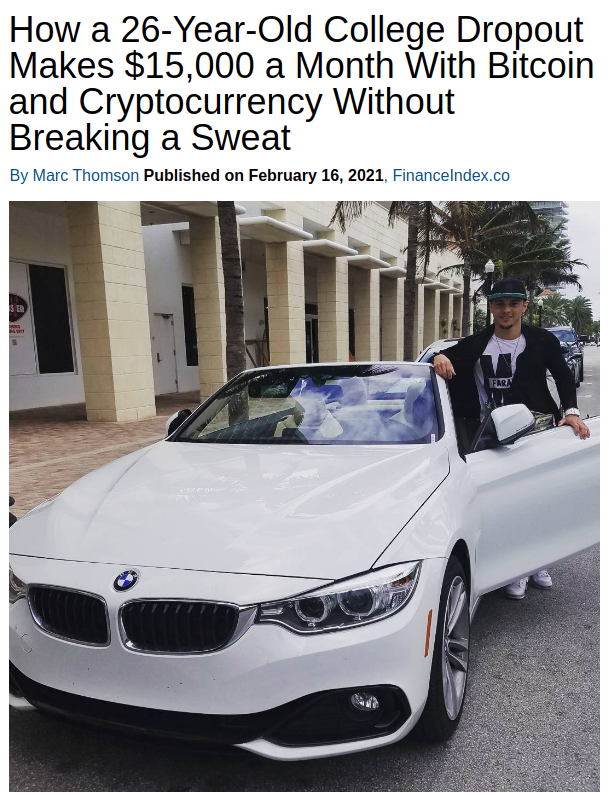
\includegraphics[scale=0.209,clip=false]{pictures/dropout.png}
    \hspace*{2ex}
    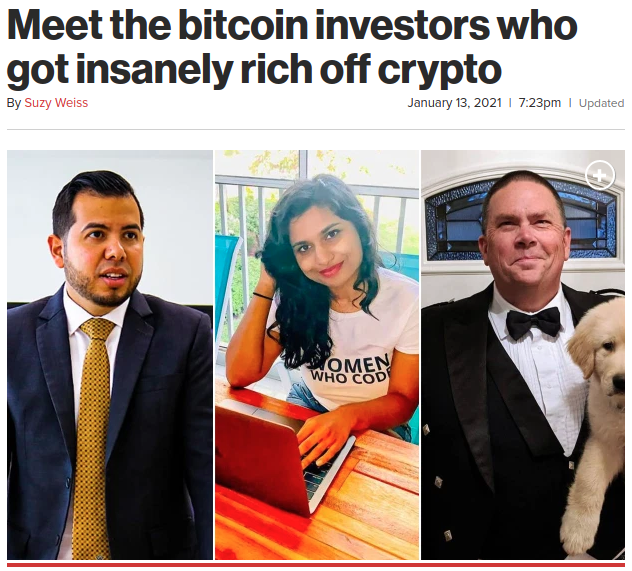
\includegraphics[scale=0.29,clip=false]{pictures/insane.png}
  \end{center}

\end{frame}

\begin{frame}\frametitle{The mainstream view of blockchain}

  \begin{center}
    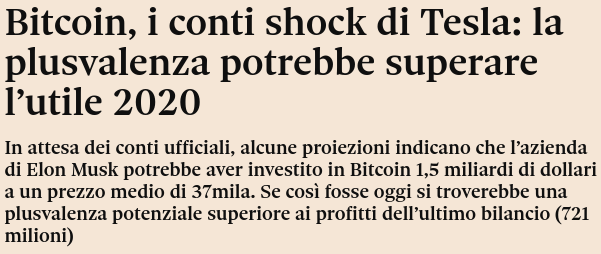
\includegraphics[scale=0.4,clip=false]{pictures/tesla.png}
  \end{center}

\end{frame}

\begin{frame}\frametitle{History}

  \begin{itemize}
  \item[1988] proof-of-work (Dwork \& Naor)
  \item[1991] a cryptographically secure chain of blocks (Haber \& Stornetta)
  \item[199x] smart contracts (Szabo)
  \item[2008] Bitcoin (Nakamoto)
  \item[2012] proof-of-stake (Peercoin)
  \item[2013] Ethereum (Buterin \& Wood)
  \item[2014] Tendermint generic proof-of-stake engine (Kwon)
  \item[2020] Ethereum 2.0 adopts the proof-of-stake
  \end{itemize}
  
\end{frame}

\begin{frame}\frametitle{Distributed network}

  \begin{center}
    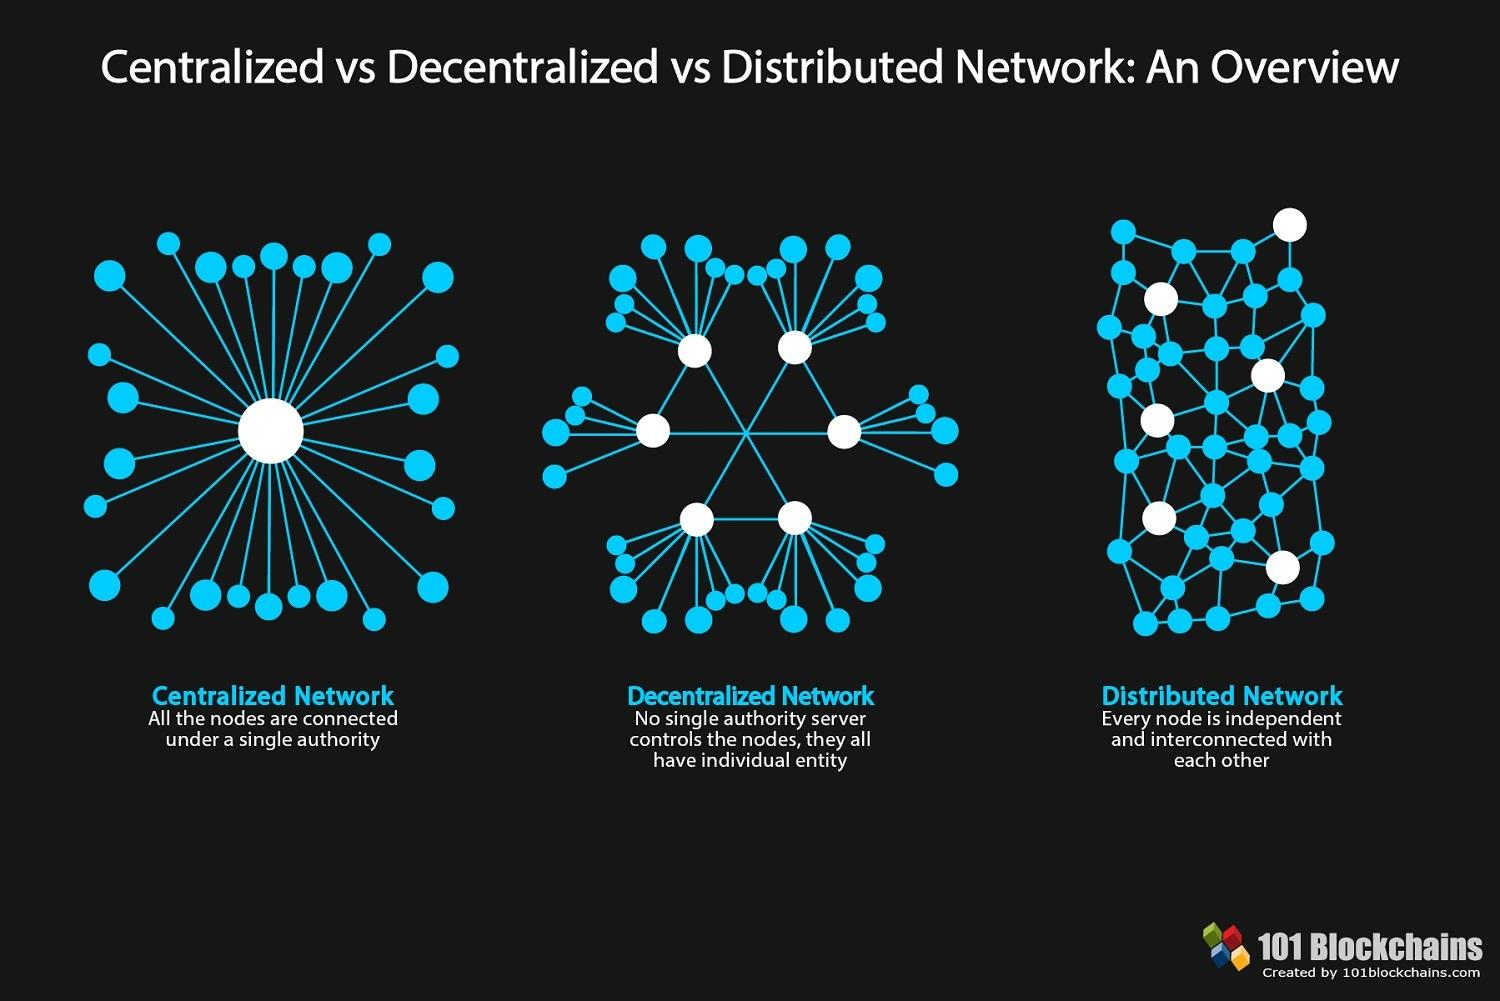
\includegraphics[scale=0.22,clip=false]{pictures/distributed.jpg}
  \end{center}

\end{frame}

\begin{frame}\frametitle{Cryptocurrencies}

  \begin{center}
    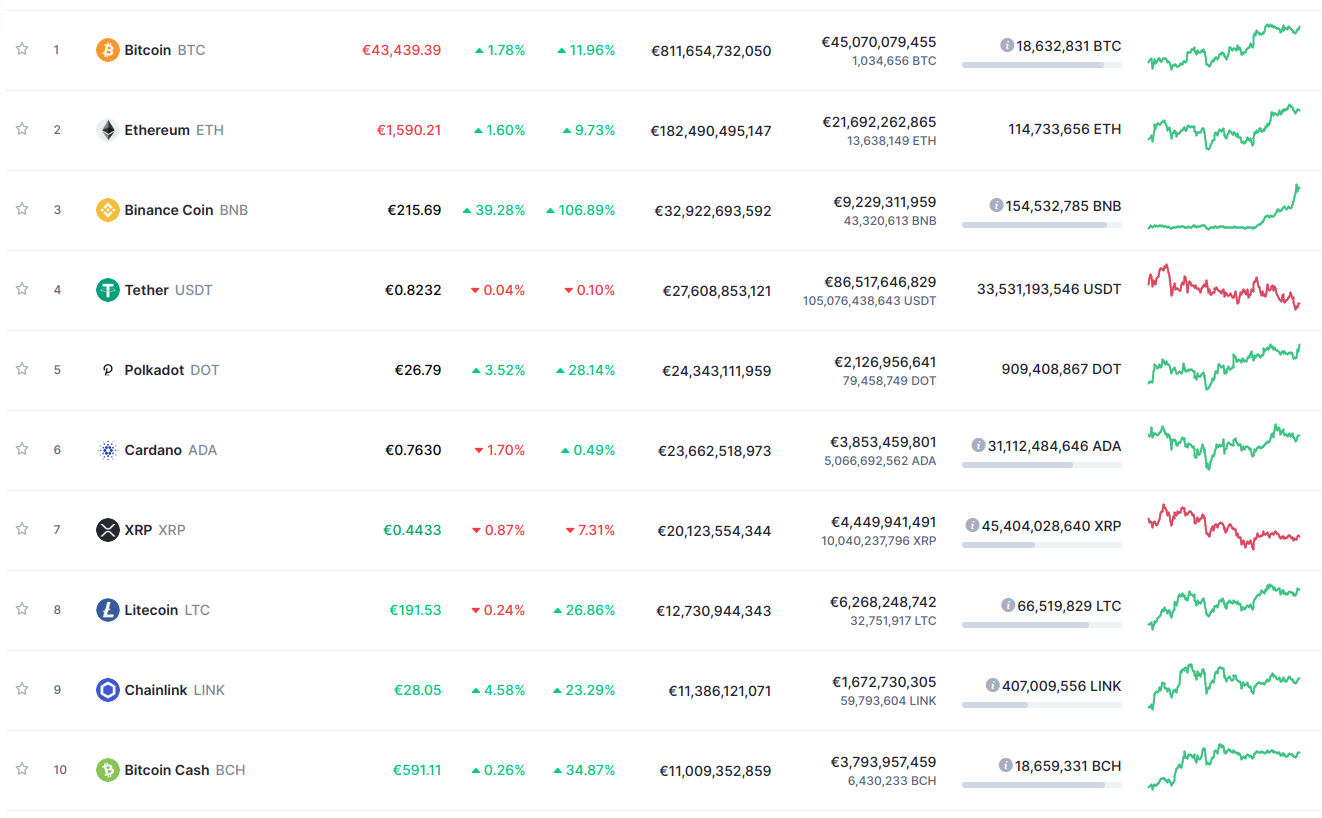
\includegraphics[scale=0.258,clip=false]{pictures/market.png}
  \end{center}

\end{frame}

\begin{frame}\frametitle{Bitcoin chart}

  \begin{center}
    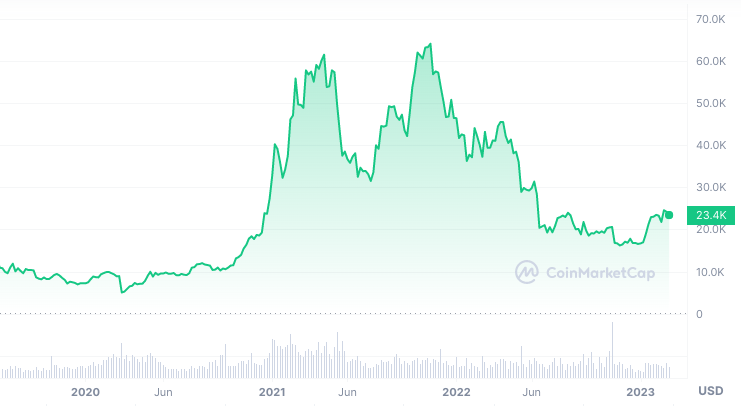
\includegraphics[width=\textwidth,clip=false]{pictures/bitcoin-coinmarketcap.png}
  \end{center}

\end{frame}

\begin{frame}\frametitle{Bitcoin capitalization (2018)}

  \begin{center}
    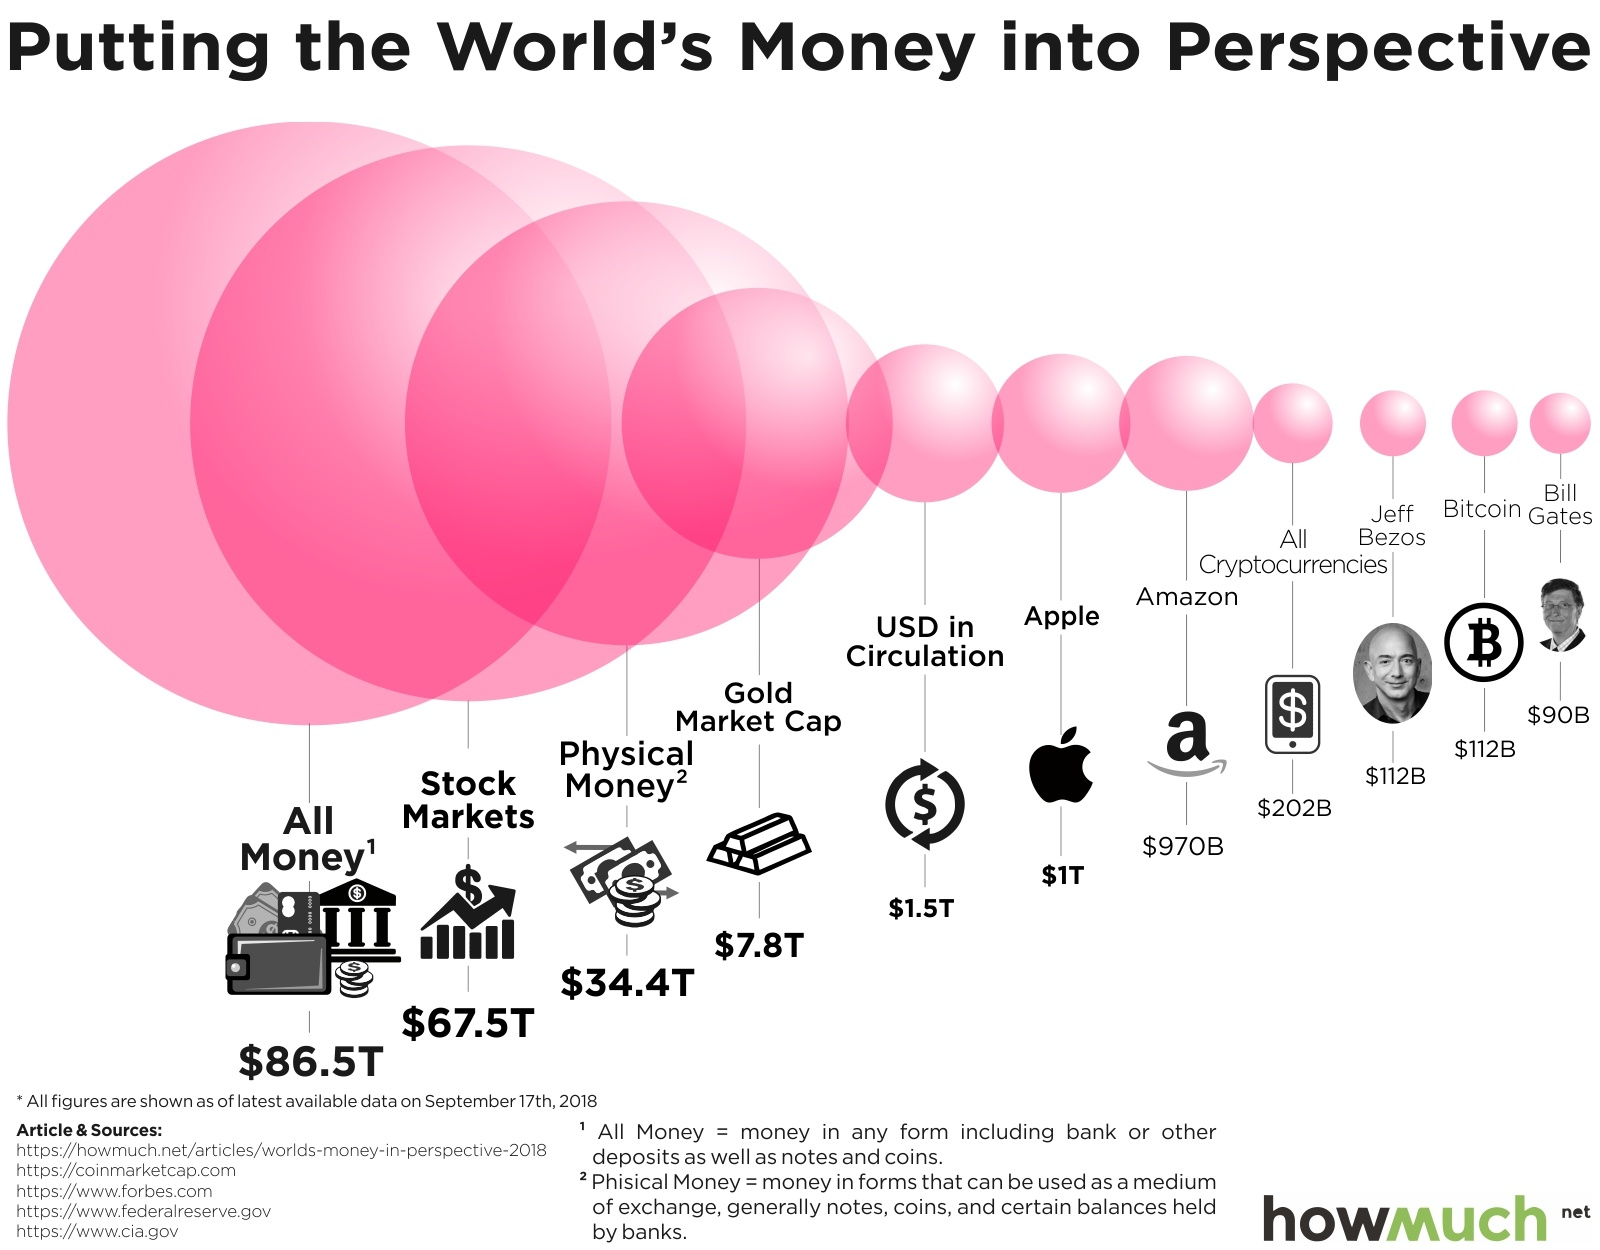
\includegraphics[scale=0.16,clip=false]{pictures/bitcoin-capitalization.jpg}
  \end{center}

  \begin{center}
    source: \url{HowMuch.net}, a financial literacy website
  \end{center}

\end{frame}

\begin{frame}\frametitle{Bitcoin transactions}

  \begin{center}
    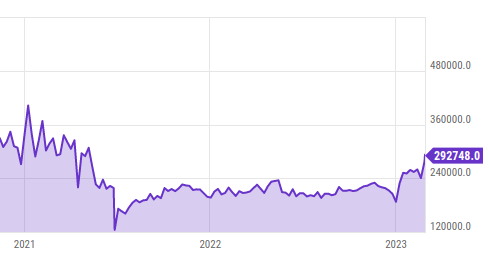
\includegraphics[scale=0.3,clip=false]{pictures/bitcoin-daily.png}
  \end{center}

  \begin{center}
    Around $300,000$ transactions per day
  \end{center}

\end{frame}

\begin{frame}\frametitle{Credit cards transactions (billions, 2018)}

  \begin{center}
    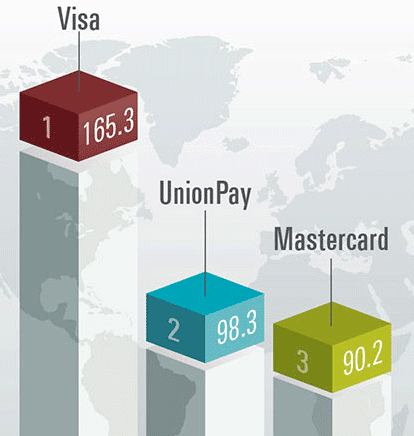
\includegraphics[scale=0.3,clip=false]{pictures/credit-cards.png}
  \end{center}

  \begin{center}
    Visa: around 451,639,000 transactions per day\\
    UnionPay: around 268,579,000 transactions per day\\
    Mastercard: around 246,448,000 transactions per day\\
    Bitcoin: around 300,000 transactions per day
  \end{center}

\end{frame}

\begin{frame}\frametitle{Bitcoin transaction fees}

  \begin{center}
    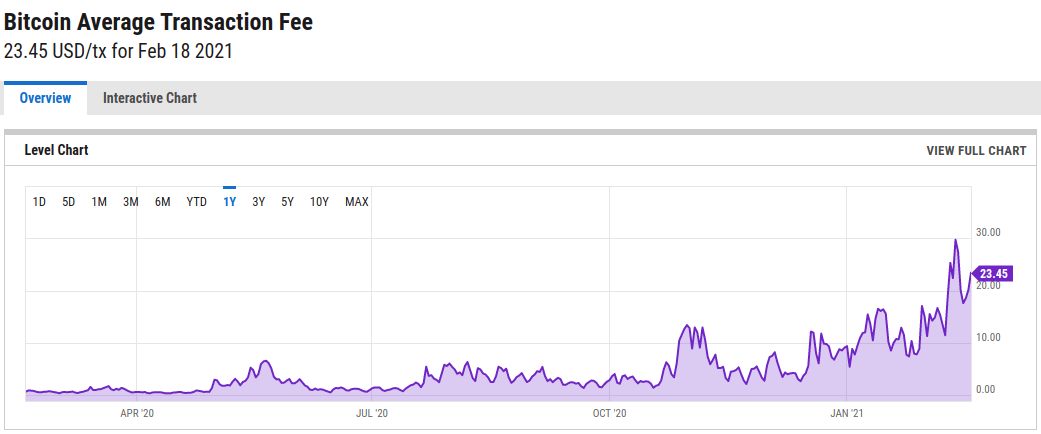
\includegraphics[width=\textwidth,clip=false]{pictures/bitcoin-fees.png}
  \end{center}

  \begin{center}
    Independent from the transacted value
  \end{center}

\end{frame}

\begin{frame}\frametitle{Credit cards transaction fees}

  \begin{center}
    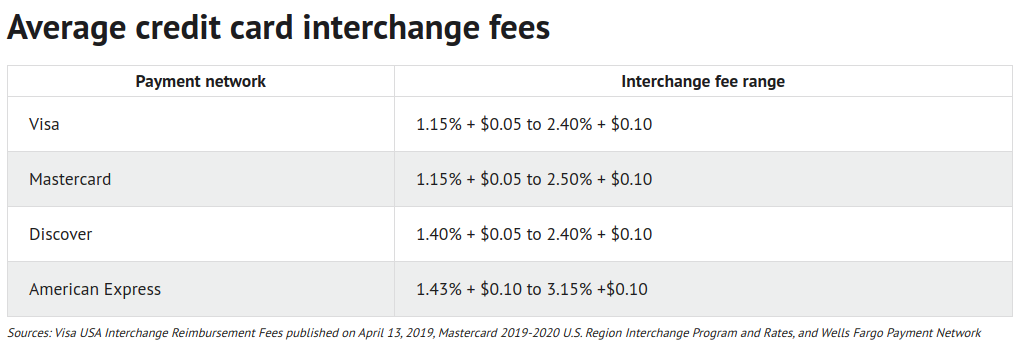
\includegraphics[width=\textwidth,clip=false]{pictures/credit-cards-fees.png}
  \end{center}

  \begin{center}
    Proportional to the transacted value
  \end{center}

\end{frame}

\begin{frame}\frametitle{The hype cycle}

  \begin{center}
    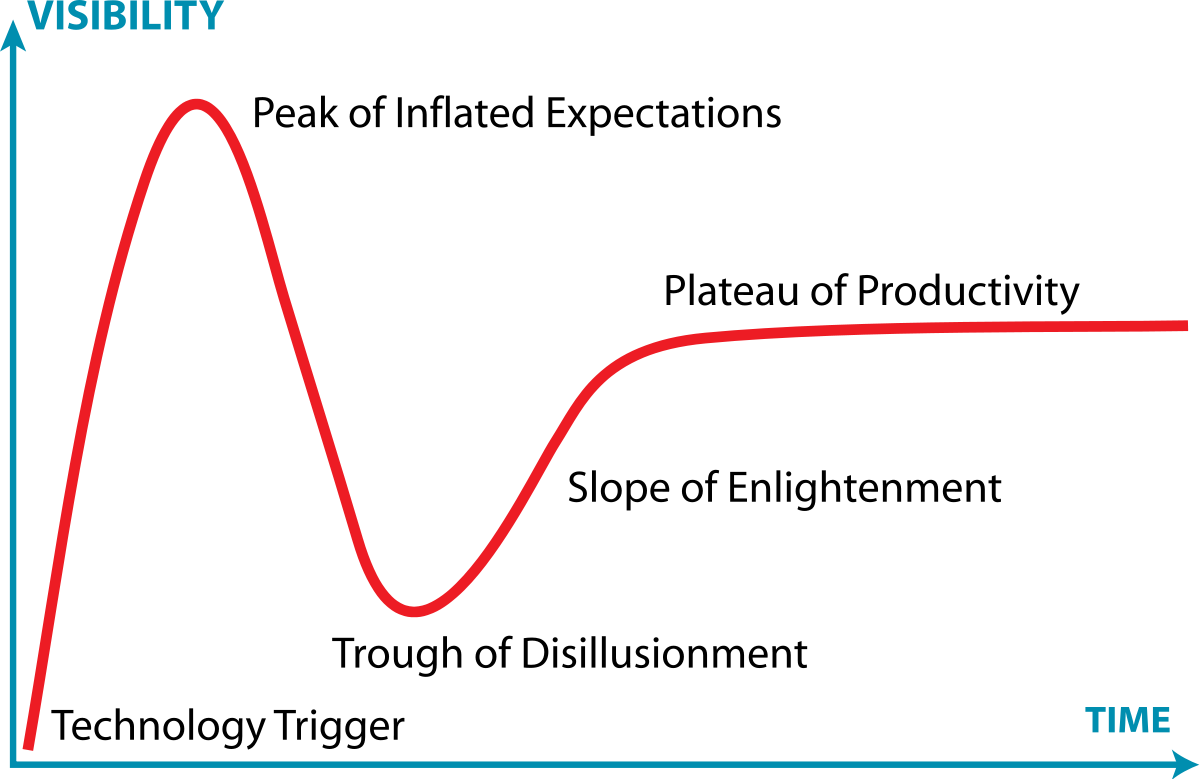
\includegraphics[width=\textwidth,clip=false]{pictures/hype-cycle.png}
  \end{center}

\end{frame}

\begin{frame}\frametitle{Beyond the hype}

  \begin{center}
    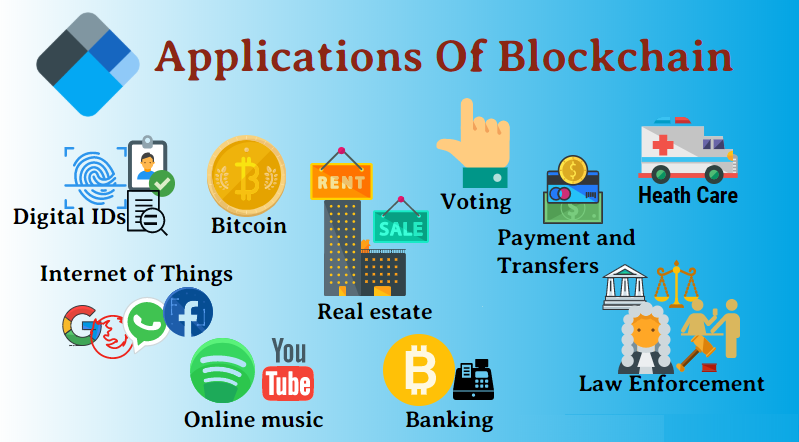
\includegraphics[scale=0.4,clip=false]{pictures/blockchain-applications.png}
  \end{center}

\end{frame}

\begin{frame}\frametitle{Beyond the hype}

  \begin{center}
    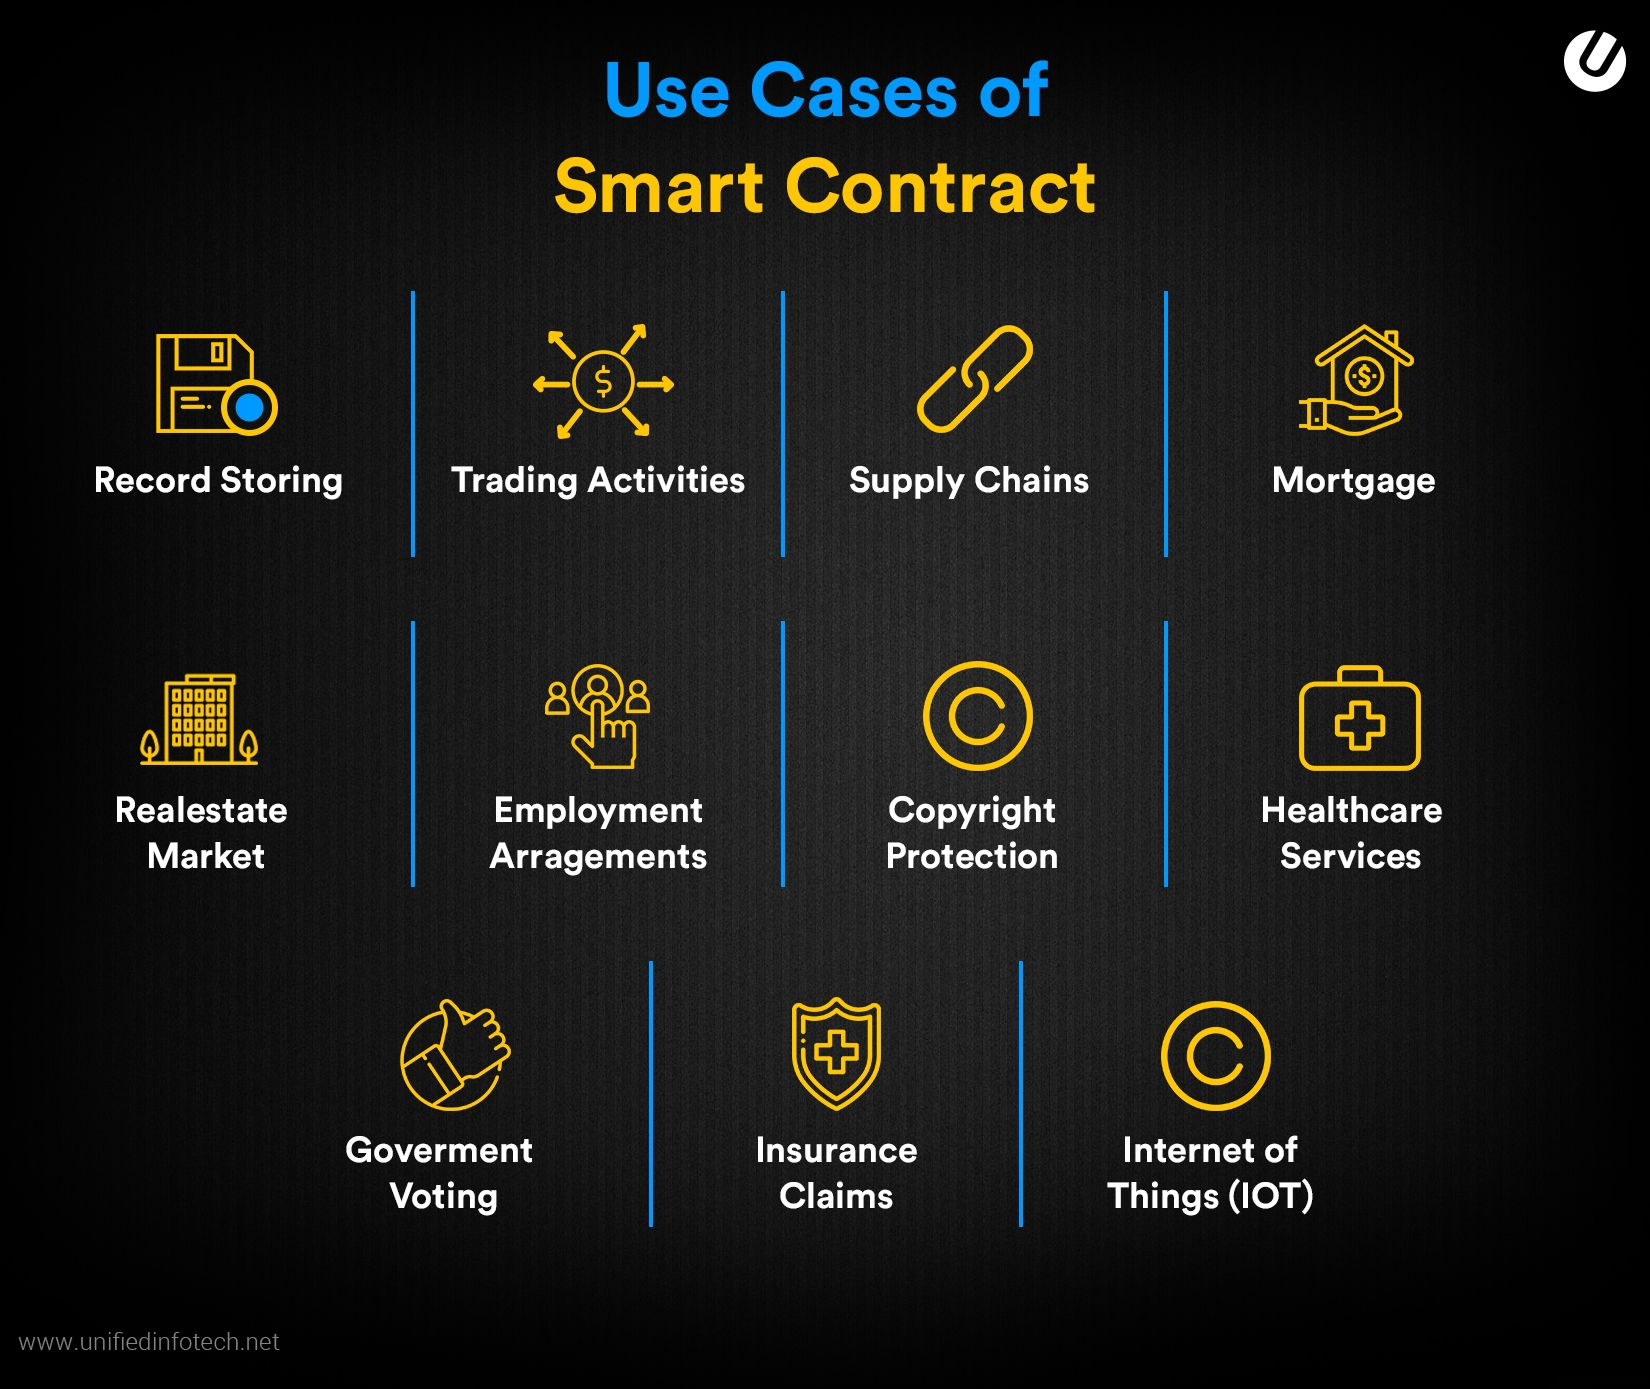
\includegraphics[scale=0.16,clip=false]{pictures/smart-contract-applications.jpg}
  \end{center}

\end{frame}

\end{document}
